% Chapter 1

\chapter{Dark Energy and Modified Gravity \label{Overview}} % Main chapter title

 % For referencing the chapter elsewhere, use \ref{Chapter1} 

%----------------------------------------------------------------------------------------

% Define some commands to keep the formatting separated from the content 
\newcommand{\keyword}[1]{\textbf{#1}}
\newcommand{\tabhead}[1]{\textbf{#1}}
\newcommand{\code}[1]{\texttt{#1}}
\newcommand{\file}[1]{\texttt{\bfseries#1}}
\newcommand{\option}[1]{\texttt{\itshape#1}}

%----------------------------------------------------------------------------------------
%

Einstein's General Relativity is the theoretical framework used in cosmology to explain the
composition and the evolution of the Universe.
The most impressive fact about this 100-year-old theory is that
when it was formulated, there was no real experimental need for it, besides maybe the
perihelion of Mercury, and it was more than a decade later, thanks to observations
by Hubble and Slipher, that physicists and astronomers where convinced that there were objects much farther away from
our galaxy and that these objects were receding away from us, with velocities proportional
to their distances. At this point the field of physical cosmology was born and the theoretical basis for it,
based on General Relativity, was developed by Lema\^{\i}tre, Friedmann, and Einstein himself among other
notable scientists.

One century later, General Relativity has passed numerous very stringent tests; from laboratory experiments (\cite{cite}) , to
low orbit tests (\cite{cite}) and solar system tests (\cite{cite}), to pulsar timing tests and the recent
exciting first detection of gravitational waves (\cite{cite}).
It is impressive that a theory that was formulated on the grounds of some very basic
principles, has proven to be so accurate across several orders of magnitude in scales.

To explain the accelerated expansion of the Universe, which was observationally verified almost 20 years ago,
(\cite{cite, supernova, 1998}), Einstein's General Relativity needs to invoke a cosmological constant, which despite the fact that
it is allowed by the theory (see Lovelock's theorem below in\cref{sub:Einstein-Hilbert} ),
possesses many unsatisfactory properties from the classical and quantum point of view. 
We will review this issue in \cref{sub:CC-problem} below.

In order to provide some context for the main results of this dissertation, we will
provide in the following sections a very brief overview of General Relativity and 
the standard cosmological model. 
In \cref{sec:GR-framework} we will review the main principles and the mathematical 
formulation of General Relativity, its field equations and
its linearized Newtonian limit.
In \cref{sec:Standard-LCDM} we will deal with the composition of the Universe,
its evolution and the standard cosmological scenario.


\section{The framework of General Relativity \label{sec:GR-framework}}

\subsection{The equivalence principle and geometry}

For Einstein, Special Relativity (SR) was unsatisfactory and didn't represent a complete theory, because it dealt with 
intertial frames and under the influence of
a gravitational field, objects would be accelerated. Moreover due to the equivalence of mass and energy in SR, 
an object with a high kinetic energy in horizontal direction would have to be accelerated differently towards the Earth, than an object
with a smaller velocity, therefore violating Newtonian observations, which claim that all test bodies experience
the same acceleration in a gravitational field, regardless of its velocity or composition.
This observation that the inertial and gravitational masses must be equivalent was of striking significance for Einstein, 
which elevated it to a guiding principle in the construction of a relativistic theory of gravity (see \cite{pais, wald, bartelmann}).

The really ingenious step was connecting this principle with differential geometry. Then, instead of the rigid 
Euclidean picture, space and time would become a dynamical 4-dimensional structure, described by differential manifolds.
Gravity would curve this space-time, but in order to maintain the equivalence principle, it is always possible to transform away gravity 
and map it to a flat Euclidean space, which is precisely one of the properties of a differentiable manifold.
If one studies the consequences of this simple principle, it leads, without the need of formulating a theory, 
to concepts like gravitational redshift and gravitational light deflection. 
Constructing from there a fully-fledged non-linear theory of gravity took Einstein more than 10 years, with the (maybe indirect) help
of very bright mathematicians like Grossmann, Levi-Civita and Hilbert.

In more modern terms, we can say that General Relativity is a theory of 
a dynamical tensor field, the metric $g_{\mu \nu}$, which defines the lengths 
of space-time intervals $ds^2 = g_{\mu \nu} dx^{\mu} dx^{\nu}$ and which is invariant under diffeomorphisms. 
All particles and fields couple to the metric $g$ in a universal way.
This means that the equations of motion and all the physical properties do not depend on the chosen coordinates.
Diffeomorphism invariance is a very important symmetry that has to be respected if one wishes to construct
extensions of gravity. 
However, at the smallest (Planck length) and largest (super-horizon) scales, there are suggestions
that this symmetry might be broken in order to be able to construct a consistent theory of Quantum Gravity
(\cite{cite Rovelli}).



\subsection{The Einstein-Hilbert action and the field equations \label{sub:Einstein-Hilbert}}

Although Einstein postulated the field equations of General Relativity in a heuristic
form, they can be obtained by varying the so-called Einstein-Hilbert action
\begin{equation}\label{eq:Einstein-Hilbert action}
S = \frac{1}{16 \pi G} \int \textrm{d}x^4 \sqrt{-g}\left( R - 2\Lambda + \mathcal{L}_m \right) \quad 
\end{equation}
with respect to the metric $g_{\mu \nu}$.
Here, $R=R^\mu_\nu$ is the Ricci scalar and $R^\munu$ is the Riemann tensor (see standard GR textbooks like \cite{wald} for its definition), 
which are functions of derivatives of the metric. The volume element is defined as $\textrm{d}x^4 \sqrt{-g}$, where
$\sqrt{-g}$ is the square root of the determinant of the metric.
Furthermore, the cosmological constant is $\Lambda$, the gravitational constant is $G$ and $\mathcal{L}_m $ is the Lagrangian of matter and radiation species.
Then the variation ($\delta S / \delta g_{\mu \nu} = 0$), yields the field equations:
\begin{equation}\label{eq:Einstein-field-equations}
G_\munu + g_{\mu \nu} \Lambda = 8 \pi G T_{\mu \nu} \quad ,
\end{equation}
where the Einstein tensor is defined as $G_\munu \equiv R_{\mu \nu} - \frac{1}{2}g_{\mu \nu} R \;$ and the 
energy-momentum tensor is defined as:
\beeqp$
T_\munu = -\frac{2}{\sqrt{-g}} \frac{\delta \mathcal{L}_m}{\delta g_\munu}
$
What \cref{eq:Einstein-field-equations} expresses is that geometry (and therefore the dynamics of the metric) is sourced by 
the energy and momentum of the fields living on this manifold.
As it was famously expressed by \cite{Misner, Wheeler, Gravitation}:
"Matter tells space-time how to curve and space-time tells geometry how to move" .

Another important property of these field equations, is that due to a purely geometric property called the Bianchi identity, which
states that the covariant divergence of the Einstein tensor is identically zero:
$\nabla_{\mu} G^\munu = 0$, 
we can ensure that the energy-momentum tensor is locally conserved:
\beeqc$
\nabla_{\mu} T^\munu = 0
$
therefore one recovers all the well-known properties of classical and fluid mechanics.

%Einstein's field equations are very complicated to solve analytically in its full glory. They consist on
%10 coupled non-linear partial differential equations.
%There are of course many interesting properties, solutions and implications of these equations, 
%which are out of the scope of this work.
%We refer the interested reader to very good textbooks like \cite{Carroll, Schultz, Misner, Thorne, Wheeler, Wald}.
%The richness and complexity of this theory is one of the reasons it has to be so successful explaining 
%star formation, gravitational collapse, black holes, gravitational waves and the evolution of the Universe.

\subsubsection{Lovelock's theorem and the uniqueness of General Relativity}

One might then ask if these field equations are unique, especially if as in our case, 
we are interested in testing these equations at the very largest scales of the Universe and we might 
be interested in modifying General Relativity in order to match current observations.
Thanks to a theorem by Vermeil and Cartan (\cite{cite Vermeil, Cartan, 1921}) 
and further simplified by Lovelock (\cite{1970, Lovelock}) we can state that in 4 dimensions,
the only divergence-free, rank-2 tensor $\mathcal{G}$, which depends on at most second derivatives
of the metric must be of the form:
\beeqp$
\mathcal{G} =  \alpha R_{\mu \nu} + \left( \Lambda - \frac{\alpha}{2} R \right) g_{\mu \nu}
$
Therefore, to ensure the correct Newtonian limit of the theory (Newtonian Poisson equation), we must set $\alpha \equiv 1$
and the proportionality constant between the Einstein tensor $G_\munu$  and the energy-momentum tensor
$T_\munu$ has to be set to $8 \pi G$.

This theorem has to fundamental implications for Cosmology.
First of all, it states that the Cosmological Constant (CC) has to appear in the classical theory of gravity,
therefore, if ---as we will see below in \cref{sub:CC-problem})--- we are not satisfied with the CC as an explanation
of the accelerated expansion of the Universe, we still have to explain why $\Lambda$ disappears from the Einstein's field equations.
Second, this theorem gives a sort of roadmap to look for modifications of gravity, which can account for the late-time expansion of the Universe.
One option is to go beyond 4 dimensions (as in DGP models \cite{DGP models}),
violate the conservation of the energy-momentum tensor with some exotic species or
add extra degrees of freedom, since with the metric alone we can't construct a more general theory.
This last option has led to the recent interest in modified gravity theories with a scalar field (see \cite{cite some scalar field}), 
with vector fields (see \cite{cite}) and with the addition of several metric (tensor) fields (see \cite{cite}). 


%----------------------------------------------------------------------------------------

\section{The standard cosmological model \label{sec:Standard-LCDM}}

The cosmological principle states
that no observer in the Universe is special and that each observer sees the Universe in the same way independently of
spatial rotations, therefore space-time has to be described by a homogeneous and isotropic metric $g_\munu$.
If furthermore, we can define a foliation of space-time, in which there is a preferred timelike direction, orthogonal
to the spatial hypersurfaces, we end up with a metric which solves the Einstein's field equations \ref{eq:Einstein-field-equations};
the so-called Friedmann-Lema\^{\i}tre-Robertson-Walker (FLRW) metric:
\beeqc$\label{eq:FLRW-full}
ds^2 = g_\munu dx^\mu dx^\nu = -dt^2 + a^2 (t) d\varsigma^2 
$
where $a$ is the scale factor, $t$ the cosmic time coordinate, and $d\varsigma^2$ is the time-independent spatial metric:
\beeqc$\label{eq:FLRW-spatial}
d\varsigma^2  = \gamma_{i j} dx^i dx^j = \frac{dr^2}{1-kr^2} + r^2(d\theta^2 + \sin^2 \theta d \phi^2)
$ 
where $r$ is the radial coordinate, $\theta$ the polar angle and $\phi$ the azimuthal angle.
The curvature $k$ which can be 0, 1 or -1, corresponds to Universes which are flat, closed or open, respectively.
Due to the stringent constraints on $k$ given by recent observations,
we will use for the rest of this work only a flat geometry with $k=0$.
Also it is standard convention that "Greek" indices run from 0 to 3, as in \cref{eq:FLRW-full},
while "Latin" indices run from 1 to 3 as in equations involving only spatial coordinates, like \cref{eq:FLRW-spatial}.




\subsection{The Friedmann equations \label{sub:Friedmann-eqs}}

The FLRW metric \cref{eq:FLRW-full} due to its scale factor, which is dependent on time, implies immediately that the Universe can expand
in its spatial coordinates. The equations describing the evolution
of the scale factor are called the \emph{Friedmann} equations. To derive them,
we need to introduce in the right hand side of Einstein's equations \cref{eq:Einstein-field-equations} an energy-momentum tensor of a perfect fluid:
\beeqc$
T^\munu = (\rho + p)u^\mu u^\nu + p g^\munu
$
which is justified since at cosmological scales, we expect the background matter in the Universe to be absent of dissipative and viscous forces.
The density $\rho$ and the pressure $p$ are the sum of the densities and pressure terms of all matter and radiation species in the universe.
If we write down now the (00) and ($i i$) components of the Einstein's field equations \cref{eq:Einstein-field-equations}, computing
the Riemann and Ricci tensors of a FLRW metric, 
we end up with two ordinary differential equations for the scale factor $a(t)$:
\beeqal$
\frac{\dot a}{a} &= \frac{8 \pi G}{3} \rho  \label{eq:Friedmann-1st}\\
\frac{\ddot a }{a} &= -\frac{4 \pi G}{3} (\rho +3 p) \label{eq:Friedmann-2nd}
$
These are the so-called Friedmann equations, which define the evolution of the Hubble function defined as:
\beeqp$
H(t) \equiv \frac{\dot a(t)}{a(t)}
$

The critical density of the Universe is defined as:
\beeqc$
\rho_{cr} = \frac{3 H^2}{8 \pi G}
$
which is the critical density that an Universe with zero curvature $k=0$ would have according to the observed value of the Hubble function.
So, for each species in the Universe, with energy density $\rho_i$, we can define the energy density fraction as:
\beeqc$
\Omega_i (t) = \frac{\rho_i (t)}{\rho_cr (t)}
$ 
so that the first Friedmann equation \cref{eq:Friedmann-1st} (for a flat Universe) can be written as:
\beeqp$
\sum_i \Omega_i (t) = 1
$

Another important quantity for each matter species is its equation of state:
\beeqc$
w \equiv \frac{p}{\rho}
$
which for species in which the pressure is not-negligible modifies considerably their dominance in the energy budget as a function of time.


\subsection{The $\Lambda$CDM model \label{sub:LCDM}}

As we have seen before, the field of Cosmology is relatively new, with less than 100 years of theoretical development
and even much less time of real observational progress.
Up to 1965?, with the discovery of the Cosmic Microwave Background (CMB) radiation by \cite{Penzias and Wilson},
cosmology was a mere speculative science. Only with the confirmation of the "Hot Big Bang paradigm" by the measurement of the radiation left over
380,000 years after the Big Bang, is that physicists started to make precise descriptions about the composition and 
the evolution of the matter species composing the Universe. The first CMB observations clarified that the Universe started
as a hot plasma of electrons, protons and photons, whose interactions in an expanding space-time matched very well the observed properties
of the present Universe.

However, there was always a piece missing in the puzzle, since the observed densities of visible matter in the Universe were too low.
For many years, there were big discussions about open and closed Universes and about invisible forms of matter.
Only with the amazing development of galaxy surveys in the 1980's and precise measurements of stars velocities in the Milky Way and other galaxies
and the development of cosmological N-body simulations in the 1990's, most cosmologists were convinced that there had to be a form of matter in the Universe
that does not interact with baryons or with electromagnetic fields, but it interacts in a standard way with gravitational fields (\cite{cite;
recent peebles, Dolag DM review, reviews, books}).
They called it "Cold Dark Matter" (CDM) because of its apparent vanishing pressure and its preference for clustering into big structures.

However, there were still some inconsistencies between the growth of structures in a pure 'CDM+baryons' model, predicted
by simulations and the observed structures in the Universe (see \cite{reviews Dolag, peacock}), so that many scientists were claiming for the addition
of a cosmological constant. However, this claims were not significant until in 1998 the teams led by \cite{Perlmutter and ..} used Supernova Type Ia
observations to prove that the Universe was experiencing a phase of accelerated expansion. This led to the re-introduction of the Cosmological Constant
and due to the theoretical problems posed by its so small observed value, to the development of a whole new 
field of research: Modified Gravity and Dark Energy.

This very rough and quick overview explains the name of the current standard cosmological model: the $\lcdm$ model. 
In this model, and according to the latest observations (see \cite{planck_collaboration_planck_2016-1})
 almost 70\% of the energy density of the Universe is composed by the Cosmological Constant
$\Lambda$, 25\% by Cold Dark Matter and less than 5\% by baryons. The remaining components are photons ---which are basically negligible today, despite the amount of light and radiation in the Universe--- and massive neutrinos,
whose mass and therefore its contribution to the "cosmic pie" has not been measured precisely enough yet.

Now we leave open the possibility that the accelerated expansion of the Universe is caused by a "Dark Energy" component, with 
an unknown equation of state $w_{DE}(z)$, where $w_{DE}(z) = -1$ would correspond to the Cosmological Constant. 
Then, together with the "standard" matter species and knowing the equation of state for each of them ($w=0$ for CDM and baryons and $w=1/3$ for radiation), we can write down
the evolution of the Hubble parameter as a function of redshift $z \equiv 1/a - 1 $ :
\beeqalsp$
H^2 (z) &= H_0 \left(  \Omega_c (1+z)^3 + \Omega_b (1+z)^3  + \Omega_r (1+z)^4   
\phantom{\exp \left[ \int_{0}^{z}  \frac{3}{1} \right]} \right. \\
      & \left.  +\Omega_{DE}  \exp \left[ \int_{0}^{z} \dx{}{\tilde z} \frac{3(1+w_{DE}(\tilde z))}{1+\tilde z} \right]     \right)
$

This is the equation that defines the background evolution of the Universe. From the Hubble function, one can obtain measurable 
cosmological distances,
the age of the Universe and the size of the observable Universe, also called the horizon.


\subsection{Distances}

Since the Universe is expanding and we measure astrophysical objects using mainly electromagnetic radiation (except after 2016 \cite{cite LIGO}, 
where Gravitational Wave Astronomy was born), it is important to define certain distances that can be measured and which are not always intuitive.
Light follows null-geodesics, so that under an FLRW metric as in \cref{eq:FLRW-full}, 
light satisfies the equation:
\beeqc$
- c dt^2 + a^2 (t) d\varsigma^2 = 0 
$
where we have recovered the speed of light $c$ to avoid confusion.
Solving for $\varsigma$ and therefore integrating this equation, defines the comoving distance $d_c$:
\beeqp$
d_c \equiv \int_0^{\varsigma_1} \mathrm{d}\varsigma = - \int_{t_0}^{t^1} \frac{c}{a(t)} \dx{}{t} 
$
Since $H = (\mathrm{d}a/\mathrm{d}t)/a = (\mathrm{d}(1/(1+z))/\mathrm{d}t)/(1/(1+z)) $, then $\mathrm{d} t = -\mathrm{d}z / ((1+z) H) $,
so that the comoving distance can be defined as:
\beeqp$
d_c (z) = \int_{0}^{z} \frac{\dx{}{\tilde z}}{H(\tilde z)}
$

\subsubsection{Angular Diameter Distance}

\subsection{The cosmological constant problem \label{sub:CC-problem}}

\begin{itemize}
\item small discussion on old and new cosmological constant problem
\item fine tuning, naturalness, basic definitions
\end{itemize}

\subsection{\revtext{Gravitational potentials}}

\begin{itemize}
	\item Gravitational potentials $\Phi$ and $\Psi$.
%	\item Very simple explanation of Gauge choice \comm{probably don't need it}
	\item Newtonian Gauge
%	\item Smallness of gravitational potentials \comm{what is this?}
	\item Remark for later that in GR $\Psi=\Phi$
	\item Weyl potential (lensing potential, null geodesics)
	\item{The Newtonian limit}
\end{itemize}



%\chapter{Dark Energy and Modified Gravity} % Main chapter title
%
%\label{DE-MG} % For referencing the chapter elsewhere

%----------------------------------------------------------------------------------------


%----------------------------------------------------------------------------------------
\section{Dark Energy and Modified Gravity \label{sec:DE-MG-sec}}


In the introduction to this work we have motivated why in the absence of a satisfactory
solution to the Cosmological Constant problem, an extension of General Relativity
is preferred in the light of present observations.
In this chapter we will deal with one of the most widely investigated solutions to the Dark Energy problem,
namely the addition of an extra dynamical degree of freedom in the form of a scalar field.

There are two basic approaches one can take at this point, either couple this field universally to all matter species, which we will call \emph{ universally-coupled theories},
or couple the field just to a specific matter component, which we will call
\emph{non-universally coupled theories}.

Universally coupled theories include Quintessence, scalar-tensor theories (ST) \cite{skordis_consistent_2009,pourtsidou_models_2013-3,clifton_modified_2012,amendola_cosmology_2013, amendola_linear_2004-7, saltas_anisotropic_2014}, Horndeski theories \cite{de2012conditions, deffayet2013formal} and Effective Field Theories of Dark Energy \cite{gleyzes_essential_2013, gubitosi_effective_2013-1, }.
We will review some of these models in \crefrange{sub:quintessence}{sub:EFT-of-DE}.
Non-universally coupled theories are in general built in such a way that baryons remain uncoupled, due to the stringent local and solar system gravity tests that constrain the scalar field--baryon coupling to be practically negligible (see \cref{sec:nonuniversal-coupling} below). In this work we will 
deal with two such theories: The Coupled Dark Energy model, which couples Dark Matter to a Dark Energy field, which will be treated in \cref{sub:CDE} and the Growing Neutrino Quintessence model, in which the neutrino mass is coupled to the ``cosmon`` scalar field, which will be the subject of \cref{sub:GNQ}.

\begin{figure}[htbp]
	\begin{center}
		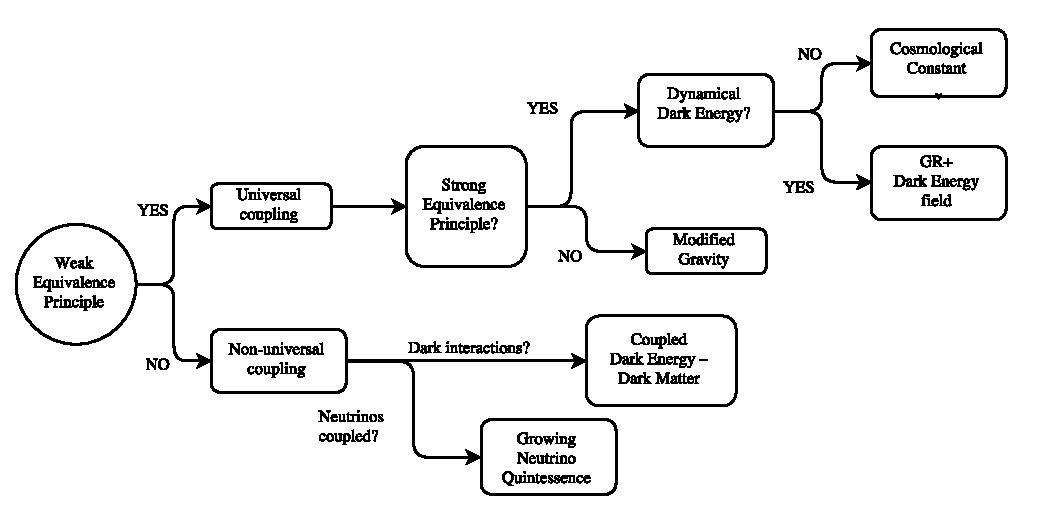
\includegraphics[width=0.99\textwidth]
		{Figures/DE-MG.pdf}
	\end{center}
	\caption[Dark Energy - Modified Gravity Flowchart]{Distinction between Dark Energy and
		Modified Gravity Theories based on the Strong and Weak Equivalence Principles (SEP and WEP), according to \cite{joyce_dark_2016-2}.
		The violation of the SEP, implies the existence of an extra fifth-force among particles, 
		or, equivalently, a modification of the standard Poisson equation. These are the so-called Modified Gravity theories.
		If the scalar degree of freedom is not coupled to matter, then we can talk about a Dark Energy model.
		In the case in which Dark Energy is not dynamical, the theory goes back to GR plus a cosmological constant.
		If the WEP is violated, then not all matter species feel the same gravitational forces and therefore
		there can be either dark sector interactions or neutrino--scalar-field interactions.
	}\label{fig:DE-vs-MG-WEP-SEP}
\end{figure}
%The term 
%Modified Gravity can encompass these but also other much more exotic modifications of GR, 
%for example involving extra dimensions and other 
%vector or tensor fields \cite{cite, bigravity, LH vector theory, dgp}. 
Furthermore, independent of the type of coupling to matter,
one can define two frames in which to study these theories. 
In the so-called Einstein frame, the action contains the standard Einstein-Hilbert term $R$,
plus a kinetic and a potential term for the scalar field $\phi$. 
However, particles are coupled to a metric that in principle depends also on the scalar field. 
On the other hand, in the Jordan frame, the scalar field $\varphi$ is non-minimally coupled
to gravity, which means that in place of the Ricci scalar,
there is a general function $f(R,\varphi)$. Besides, one can also have a potential
and kinetic term for the scalar field. 
The Einstein-Hilbert term is modified, but particles feel a metric that is purely of geometrical origin. 
We will specify the equations for these two different frames in
\cref{sec:Einstein-Jordan} below.
%but 
%One can regard this extra degree of freedom as an exotic new form of matter, affecting the right hand side of the Einstein field equation \ref{eq:Einstein-field-equations} and generally coupled in distinct ways to different matter fields, 
%or one can consider gravity to have an extra degree of freedom coupled non-minimally to the 
%Ricci scalar and therefore modifying 
%directly the left hand side of Einstein's field equations. The latter frame of reference
%is called the Jordan frame, while the former is usually called the Einstein frame.

%For theories in which all matter fields are coupled in the same way to the scalar field, both descriptions
%have to be equivalent and we call them \emph{universally coupled} theories. 
%For theories in which the coupling is specific to a matter field (i.e. neutrinos), the theory 
%is usually formulated in the Einstein frame. These are the so-called \emph{non-universally} coupled theories.
%In the following, we will use this classification to discuss the models studied in this work.

The distinction between Modified Gravity and Dark Energy is somewhat diffuse, since as mentioned above, 
an exotic form of matter in the Einstein's equations can always be considered as a modification 
of involving geometry. However, we will use a definition introduced recently by \cite{joyce_dark_2016-2}, 
which is quite practical in terms of its observable properties. 

In this definition, Dark Energy encompasses models which respect both the Weak and the Strong Equivalence
Principles and therefore do not involve extra fifth-forces that act between particles besides gravitational 
interactions (and the other three fundamental forces of nature). 
Modified Gravity encompasses models where the Strong Equivalence Principle is violated and therefore 
bodies can have an extra "scalar charge" that leads to the appearance of a fifth force among them.
In non-universally coupled theories, the Weak Equivalence Principle is violated,
since test bodies would feel different accelerations depending on
their composition. Usually, in these models baryons are uncoupled and therefore they might be called ``dark sector interaction`` theories.


The term ``modified gravity`` is also more general and it is used for
any theory beyond GR that is able to explain the cosmological history
of the Universe. This can include extra dimensions \cite{deffayet2002accelerated},
massive bimetric gravities \cite{akrami2015bimetric, konnig2014stable} or Lorentz-violating theories
\cite{blas2011models}. However, these models are out of the scope of this dissertation. 
For the rest of this work, when we mention Modified Gravity, we will refer to our definition according
to our discussion above and the diagram \ref{fig:DE-vs-MG-WEP-SEP}.

%In the first \cref{sec:universal-coupling} we will discuss universally coupled theories, which include ---among many others--- Quintessence, f(R),
%Scalar-Tensor theories and the Horndeski theory 
%(see \cite{Luca, Cliffton, Silvestri, Joyce, and more} for comprehensive reviews on Modified Gravity theories). 
%We will also discuss
%more general modifications of gravity which are based on the Effective Field Theory (EFT) approach to
%Dark Energy and parameterizations of modifications of gravity, which
%are not connected to any particular model and can accommodate any deviation from standard GR, at least at the linear 
%level in perturbation theory.
%
%In the second section, we will deal with two specific non-universally coupled models of dark energy used in this work. 
%The first one is
%called Coupled Dark Energy (CDE), which only couples the DE field to dark matter particles and leaves baryons uncoupled, therefore respecting solar system
%constraints on gravity.
%The second one, called Growing Neutrino Quintessence (GNQ), is a model in which the neutrino mass is coupled to the DE scalar field, while 
%all other species remain uncoupled, which is a very phenomenologically rich theory, but possesses theoretical difficulties due to its highly non-linear evolution.
%We will explain the motivations for each of these models and we will emphasize their differences in the predictions for structure formation and the background evolution of the Universe.
 
\section{The Einstein and the Jordan frames \label{sec:Einstein-Jordan}}

In this section we will review the form of the action for scalar-tensor theories in the Einstein and Jordan frames,
which are going to be useful concepts in the following chapters. For the moment we will work in units where the reduced Planck mass
$M_{Pl}^{2} = 1/(8 \pi G)$ is equal to unity.

A scalar-tensor theory can be formulated in the "Jordan frame" as:
\beeqalsp$\label{eq:jordan-frame-action}
\mathcal{S} =& \int \dx{4}{x} \sqrt{-g} \left[  \frac{1}{2} F(\varphi, R) - \frac{1}{2} K(\varphi) g^{\mu \nu}  \partial_{\mu}\varphi \partial_{\nu}\varphi 
- U(\varphi)    \right]  \\
& -\int \dx{4}{x} \sqrt{-g} \mathcal{L}^i_m (g_{\mu \nu} , \varPsi^i_m \zeta^{i}(\varphi)) \quad ,
$
where an index $i$ in the matter sector stands for each of the matter species in the Universe. 
In the case of universal coupling, all matter species ``feel`` the same metric $g$, 
 and are are coupled in the same way to the scalar field, through the function
 $\zeta^{i}(\varphi)$. 
In this frame, the Ricci scalar is non-minimally coupled to the field $\varphi$ through a function $F(R, \varphi)$ and, in general, 
can also contain a potential term for $\varphi$ with an extra function $K(\varphi)$ multiplying the kinetic term of the scalar field.
Matter particles follow the standard geodesics of GR and the energy momentum tensor of the matter species is covariantly conserved.

We can relate the Jordan to the Einstein frame, by doing a conformal transformation of the metric $g$, where
this transformation is defined as:
\beeqc$
\tilde{g}^{(i)} = \Omega^2(\phi, R) g
$
and $\Omega^2(\phi, R)$ is a function of the scalar field and ---in the most general case--- of the Ricci scalar, given by
\beeqp$
\Omega^2(\varphi,R) \equiv \parder{F}{R} 
$
Then, the scalar-tensor action in the `Einstein-frame` takes the following form:
\beeqc$\label{eq:einstein-frame-action}
\mathcal{S} = \int \dx{4}{x} \sqrt{-\tilde{g}} \left[  \frac{1}{2} \tilde{R} - \frac{1}{2} \tilde{g}^{\mu \nu}  \partial_{\mu}\phi \partial_{\nu}\phi 
- V(\phi)    \right] - \int \dx{4}{x} \sqrt{-\tilde{g}} \mathcal{L}^i_m (\tilde{g}^{(i)}_{\mu \nu} , 
\varPsi_m^{(i)} \tilde{\zeta}^{i}(\phi) )
$
where a tilde stands for the conformally transformed quantities.
In the case of universal coupling (see \cref{sec:universal-coupling} below), all matter species would couple to the same function $\tilde{\zeta}^{i}(\phi)$. 
If there is non-universal coupling (see \cref{sec:nonuniversal-coupling} below) each species would
have a different function $\tilde{\zeta}^{i}(\phi)$ or be totally uncoupled from the
field with $\tilde{\zeta}^{i}(\phi) = 1$. 
The Einstein frame is defined as the 
frame in which the gravitational part of the action looks standard, since the Ricci scalar appears without multiplicative factors.
In this formulation, the energy-momentum $T^{(m)}_{\mu \nu}$ of the coupled matter species is not conserved, but rather
the sum of the energy momentum tensor of matter and the scalar field $T^{(m+\phi)}_{\mu \nu}$ is the conserved quantity.

For non-relativistic particles this field dependent function $\zeta(\phi)$ can be also absorbed into the mass $m=m(\phi)$, giving rise to particles with varying mass, as we will see below.
This field dependent mass can also be linked to an extra "fifth-force", 
with a coupling strength $Q$
defined by:
\beeqc$\label{eq:definition-of-coupling-Q}
Q(\phi) \equiv -\frac{1}{2}\frac{\partial \ln f}{\partial \phi}
$
where, in these theories, the function $F$ above takes the form: $F(\varphi, R) = f(\varphi)R-2U(\varphi)$, where
$f$ and $U$ are free functions of the field.
To go from the Jordan frame action \cref{eq:jordan-frame-action} to the Einstein frame action
\cref{eq:einstein-frame-action} and at the same time keep a \emph{canonical} kinetic term,
($1/2 \nabla^2 \phi$), a field redefinition has to be performed:
\beeq$
\phi = \int \dx{}{\varphi} \sqrt{(3/2)(f_{,\varphi}/f)^2 + K/f}
$
where the potentials $U$ and $V$ are related by $V = U/f^2$.


For non-universal coupling, we will see two examples of theories formulated in the Einstein frame in \cref{sub:CDE} and \cref{sub:GNQ}.
In \cref{sub:CDE} we will see an example of a constant coupling and in \cref{sub:GNQ} we will see an example of a field-dependent coupling, 
giving rise to very different phenomenologies.

For conformally-invariant theories (those theories in which null-geodesics are not modified by conformal transformations), the conformal factor
just depends on the scalar field and can be written as $\Omega^2(\varphi)=\exp(2\varphi)$. 
This can be seen by performing the transformation $g \rightarrow e^{2\varphi} g$ and 
observing that, at first order in the
scalar field and the gravitational potentials, $\Phi \rightarrow \Phi-\varphi$ and $\Psi \rightarrow \Psi+\varphi$, leaving 
the Weyl (lensing) potential $\Phi_{\rm Weyl} = (1/2)(\Psi + \Phi)$ invariant.
These theories are interesting, since they do not affect gravitational lensing observations,
but still can provide interesting non-standard features in the clustering of matter.


We have to emphasize that physical measurable quantities have to be frame-independent by definition,
since this frame transformation amounts to nothing more than a coordinate and field redefinition 
and one of the principles of the GR formalism which we are not abandoning
is diffeomorphism invariance, which ensures that 
the theory is invariant under general coordinate transformations.


\section{Universal coupling to matter \label{sec:universal-coupling}}

Scalar-tensor theories with universal coupling written in the Jordan frame \cref{eq:jordan-frame-action}, 
encompass many of the most widely studied dark energy and modified gravity models in the literature. 
For example, $f(R)$ theories \cite{de2010f} are recovered when $F(R,\varphi) = f(R)$ and $K=0$;
Brans-Dicke theory \cite{brans1961mach} is recovered when $F(R,\varphi) = \varphi R $ and 
$K(\varphi) = \omega_{BD}/\varphi$, where $\omega_{BD}$ is the Brans-Dicke parameter and finally "k-essence" 
\cite{armendariz2001essentials} is the case in which $F(R,\varphi) = R$ and $K$ can be a general
function of $\varphi$ and its kinetic term $(\nabla \varphi)^2$. 

There are also other theories of modified gravity with a scalar field, that are not encompassed in the set of "scalar-tensor"
theories and that have gained a lot of attention recently. Namely, Galileons \cite{deffayet2011k}, Horndeski \cite{deffayet2013formal} 
and Beyond-Horndeski theories \cite{gleyzes2015exploring}. 
These theories are universally coupled to matter, are formulated
in the Jordan frame and cannot be expressed in the Einstein frame by a conformal transformation, since they contain much more complicated
derivative interactions, for example free functions of $\Box \varphi$ (see \cite{zumalacarregui2014transforming}), where the ``box operator`` is defined as $\Box \equiv g^{\munu}\partial_{\mu}\partial_{\nu}$.

Horndeski's theory \cite{horndeski_original} is an interesting case, since it is the most general theory of 
a scalar field coupled to a metric, with second order equations of motion and free of ghost instabilities. 
This theory was first formulated by Horndeski in the 1970's \cite{horndeski_original}, in a purely mathematical way and was re-discovered by \cite{deffayet2013formal}
and others, at the beginning of the present decade, in the context of Galileon scalar fields. The simplest Galileon model, the so-called cubic Galileon, has a Lagrangian of the form:
$\mathcal{L} \propto R/2 - (\partial \varphi)^2 - (1/\Lambda_3)\Box \varphi (\partial \varphi)^2$, 
where $ \Lambda_3 $ is a free scale that can be set in the theory. The term Galileons, comes from the fact that
these theories are the more general theories, which are invariant under a general Galiliean transformation of the field $\varphi \rightarrow \varphi + b_\mu x^\mu +c$.
Beyond-Horndeski theories are extensions of Horndeski that have higher than second order equations of motion, when expressed 
in the Newtonian gauge, but where the propagating scalar degree of freedom still obeys second order differential equations, avoiding
instabilities, see
\cite{gleyzes2015exploring} and \cite{zumalacarregui2014transforming} for more details on this direction of research.

For the purposes of this work, we will now detail one of the oldest models of Dark Energy, namely
the Quintessence model \cite{ratra_cosmological_1988, wetterich_cosmology_1988} and its extension
Coupled Quintessence introduced by \cite{Amendola_2000}.

Later on we will deal with general modifications of gravity, whose
effect on structure formation can be parameterized by two functions of
scale and time. Finally we will shortly explain one of the most general approaches
to construct theories of modified gravity at linear order; the so-called Effective Field Theory of Dark Energy. We will show also its connection to Horndeski's theory.

\subsection{Quintessence \label{sub:quintessence}}

The Quintessence model
%, which takes its name from the Latin word for "fifth element"
%is one of the oldest models of Dark Energy. It 
was introduced by several authors almost 30 years
ago \cite{ratra_cosmological_1988, wetterich_cosmology_1988},
motivated by studying the 
breaking of scale invariance, which could give rise to a dynamical cosmological constant.
Its Lagrangian is of the form \cref{eq:jordan-frame-action}, with
$F(\varphi, R) = R$, $K = 1$ and a potential $U(\varphi)$.
Since this is a homogeneous field without couplings, we can find its energy density and its pressure 
straightforwardly from the energy-momentum tensor of a perfect fluid in a FLRW background:
\begin{align}\label{eq:quintessence-rho-p}
&\rho_{\varphi} = -T^{0 (\varphi)}_0 = \frac{1}{2}\dot\varphi^2 + U(\varphi) \quad 
&p_{\varphi} = \frac{1}{3} T^{i (\varphi)}_i = \frac{1}{2}\dot\varphi^2 - U(\varphi) \quad ,
\end{align}
which yields the equation of state:
\beeqp$
w_\varphi  = \frac{p_{\varphi}}\rho_{\varphi} = \frac{\dot\varphi^2 - U(\varphi)}{\dot\varphi^2 + U(\varphi)}
$
We can see that for obtaining the required behavior of $w\approx -1$ at late times, in order to fit 
the observations of the expansion of the Universe, we need that the kinetic term $\dot\varphi^2$
becomes much smaller than the potential term $U$.
From the continuity equation for a perfect fluid or from the variation of the action with respect to $\varphi$,
we can find the Klein-Gordon equation for this field:
\beeqp$
\label{eq:Klein-Gordon-Quintessence}
\ddot \varphi + 3 H \dot \varphi + U_{,\varphi} = 0
$
The dynamics and the phenomenology of this model are entirely determined by the shape of the potential
and for this there are many possibilities (see \cite[chap. 7]{amendola_dark_2010}, for a comprehensive review).
The most interesting solutions, which can alleviate the cosmological coincidence problem, are those in which the field
tracks the evolution of matter at early times ($w_\varphi \approx 1$) and then 
evolves towards an attractor (effectively being independent of initial conditions) 
at late times, which yields cosmic acceleration with $w_\varphi \approx -1+\xi$.
The parameter $\xi$ is a combination of parameters entering the potential function $U(\varphi)$ and allows
to distinguish Quintessence from a simple cosmological constant at present time.
The most studied potentials are the exponential potential $U(\varphi) = U_0\exp(-\lambda \varphi)$ 
(see \cite{copeland_exponential_1998}), where $\lambda$ is a free parameter
and the inverse power-law potential $U(\varphi) = M^{4+n} \varphi^{-n}$,
where $M$ is a mass scale of the theory.

Due to the so low energy density of dark energy ($\rho_{DE} \approx 10 ^{-120} M_{Pl}$)
compared to typical energies appearing in particle physics, it is not so easy to construct a 
viable model of Quintessence which is motivated by a fundamental theory. Nevertheless, there are 
some succesful approaches like fermion condensates, Pseudo-Nambu-Goldstone models and 
dilatonic quintessence (see \cite{amendola_dark_2010} and references therein).
These models have to satisfy that at present times dark energy is the dominating 
energy density in the Universe and therefore from the Friedmann equation and \cref{eq:quintessence-rho-p}:
\beeqp$
U(\varphi_0) \approx H_0^2 M_{Pl}^2
$
If we take an inverse power law potential, $U(\varphi) = M^{4+n} \varphi^{-n}$, and take the field to be at present $\varphi_0 = M_{Pl}$,
this would yield a mass scale $M$ of the order
of:
\beeqc$
M \approx H_0^{2/(4+n)} M_{Pl}^{(2+n)/(4+n)}
$
where, with $H_0 \approx 10^{-42} \mathrm{GeV} $, we get a mass scale of $M \approx 10^{-1} \mathrm{GeV}$
for $n=2$, which is a scale compatible with Standard Model particles.
Moreover, to satisfy the requirement of acceleration today, 
the slow-roll condition (analogous to the one in inflation \cite{bartolo_non-gaussianity_2004}) must satisfy 
$ \frac{M_{Pl} V_{,\varphi \varphi}}{V(\varphi_0)} \lessapprox 1$.
Defining the mass of the scalar field $m_\varphi$ as the second derivative of the potential with respect to the field,
$m^2_\varphi \equiv  V_{,\varphi \varphi} $, yields a condition for the scalar field mass:
\beeqp$
m_\varphi \lessapprox H_0 \approx 10^{-33} \mathrm{eV}
$
So in order to be compatible with observations, 
the scalar field mass must be extremely small.
This could cause problems for quintessence models,
since the stability of such small masses is not always guaranteed under radiative corrections \cite{kolda1999quintessential}.

\subsection{Coupled Quintessence \label{sub:CQ}}

It is also interesting to observe the effects of a coupling between the 
scalar field and the matter species.
In \cref{eq:definition-of-coupling-Q} we already saw how from a general
Scalar-Tensor theory, a coupling between matter species and 
the field can arise from an action like the one in \cref{eq:jordan-frame-action}.
However, the matter equations of motion and the Klein-Gordon equation become more tractable if
we make a conformal transformation into the Einstein frame, where
the scalar field Lagrangian will be canonical, but matter will
be coupled to a metric that contains a function of the field $\phi$.
In this case, as stated before, the individual energy-momentum tensors will not
be conserved:
\beeqal$\label{eq:Tmunu-for-CQ}
&\nabla_{\mu} T^\mu_{\nu (\phi)} = -Q T_m \nabla_{\nu}\phi \quad & \nabla_{\mu} T^\mu_{\nu (m)} = +Q T_m \nabla_{\nu}\phi \;\;,
$
where $Q$ is the coupling function and $T_m$ the trace of the energy-momentum tensor of matter. Through the 
conformal transformation the field should also be coupled to radiation, since radiation also feels gravity, 
but since the trace of the energy-momentum tensor of radiation vanishes identically, it does not appear in the 
conservation equations.
In general,
the coupling $Q$ can be different for baryons and for dark matter.
The coupling to baryons is severely constrained by local gravity experiments (see \cite{Agashe:2014kda})
and therefore uncoupling the baryons from the theory 
can yield a model compatible with observations as we will see below for the Coupled Dark Energy model in \cref{sub:CDE}.

If all matter fields are coupled, then some screening mechanism
has to be invoked in order to pass the stringent Solar System and local gravity constraints.
One possibility is the chameleon mechanism (see the book by \citetitle{amendola_dark_2010}, for a comprehensive review), which
is a coupled quintessence field whose effective potential (and therefore its effective mass)
changes according to the environment it is in.
These kind of theories can arise from an action like in \cref{eq:jordan-frame-action},
with $F(\varphi,R) = \exp(-2Q\varphi)R$ and $K(\varphi) =(1-6Q^2)\exp(-2Q\varphi)R$.
For each distribution of matter, taken to be spherically symmetric for simplicity, 
one has to calculate the profile of the field $\varphi (r)$ as a function of the radius $r$,
and one can tune the parameters in such a way that the effective coupling $Q_{\rm eff}$
in a certain region is much smaller than the bare coupling $Q$ appearing in the action.
In this way one can recover for star systems and galaxies the Newtonian predictions.
For more details on these calculations, see \cite{amendola_dark_2010}, chapter 8.4.



\subsection{Effective Field Theory of Dark Energy and Horndeski Theory \label{sub:EFT-of-DE}}

Until now we have treated Dark Energy and Modified Gravity in a rather phenomenological way,
adding a scalar field with an kinetic term, a coupling and a potential without a clear understanding
of which terms are allowed or not.
Recently, there have been substantial efforts by many authors to build an effective field theory 
of dark energy and modified gravity that encompasses all possible terms that are allowed 
in the action at second order (see \cite{Gubitosi2013, Gleyzes2016, bloomfield_dark_2013}). Considering only one extra dynamical
scalar field, respecting the symmetries of homogeneity and isotropy and following the Weak Equivalence Principle (WEP),
this theory can be uniquely formulated. Its action in the Jordan frame (and written in conformal time $\tau$) takes the form:
\begin{align}\label{eq:EFT-action}
\begin{split}
S ={}& \int \dx{4}{x} \sqrt{-g} \left[ \frac{M_{Pl}^2}{2} [1 + \Omega(\tau)] R + \Lambda(\tau) -a^2 c(\tau)\delta g^{00} \right. \\
     & + \frac{M_{2}^4 (\tau)}{2}(a^2 \delta g^{00})^2 -\bar{M}_{1}^3 (\tau) 2 a^2 \delta K^\mu_\mu \delta g^{00} \\
     & - \frac{\bar{M}_2^2 (\tau)}{2} (\delta K_\mu^\mu )^2 - \frac{\bar{M}_3^2 (\tau)}{2}\delta K^{\mu}_{\nu}\delta K^{\nu}_{\mu} \\
     & + a^2 \frac{\hat{M}^2 (\tau)}{2} \delta g^{00} \delta R^{(3)} \\
     & + m^2_2(\tau) (g^{\mu \nu} + n^\mu n^\nu) \partial_{\mu} (a^2 g^{00})\partial_{\nu} (a^2 g^{00}) \\
     & \left. + \mathcal{L}_m(g_{\mu \nu}, \varPsi_m) \right] \quad.
\end{split}
\end{align}
To construct this action, the spacetime has been foliated (similarly to the 3+1 ADM decomposition) into a time direction
and spatial hypersurfaces that coincide with the uniform scalar field hypersurfaces (this is the so-called unitary gauge). 
The preferred time direction is then (c.f. \cite{Gubitosi2013})
\beeqc$
n_\mu \equiv -\frac{\partial_{\mu}\phi}{\sqrt{-(\partial \phi)^2}}
$
which induces a spatial metric $h_{\mu \nu} \equiv g^{\mu \nu} + n^\mu n^\nu $, a spatial Ricci scalar $R^{(3)}$
and defines an extrinsic curvature:
\beeqp$
K_{\mu \nu} \equiv h^{\sigma}_{\mu} \nabla_{\sigma} n_\nu
$
The rest of the terms in the EFT action \cref{eq:EFT-action} are nine free functions of time:\\
$\{\Omega(\tau), \Lambda(\tau), c(\tau), M_{2}^4 (\tau), \bar{M}_{1}^3 (\tau), \bar{M}_2^2 (\tau), \bar{M}_3^2 (\tau),
 \hat{M}^2 (\tau), m^2_2(\tau)\}$, whose choice specify the theory.
This theory encompasses all theories of an extra dynamical scalar field, which respect the WEP.
At the linear level in perturbations, it includes the Horndeski theory (mentioned above in \cref{sec:universal-coupling}) 
and also theories which go beyond second order equations of motion (in the Newtonian gauge), also called
Beyond-Horndeski theories (see \cite{gleyzes2015exploring})

Since these theory involves many free functions, we need to choose a parametrization for each of them and 
we need to take some simplifying assumptions in order to be able to constrain this theory with data.
Recently, a code capable of calculating the linear Einstein-Boltzmann system of equations for the EFT formalism
has been made public, the so-called \textsc{EFTCAMB} (\cite{hu_effective_2014, hu_eftcamb/eftcosmomc:_2014-2}), which is based 
on the widely used \textsc{CAMB} code by\cite{lewis_efficient_2000}. 
We will use this code to calculate the observables which we will 
implement into our Fisher forecast in \cref{sec:EFT-forecasts}.

Furthermore, we will use the assumptions taken in \cite{planck_collaboration_planck_2016} in order to simplify
the theoretical modeling.
If we assume a $\lcdm$ background, and choose freely a function
$\Omega(\tau)$, the functions $\Lambda(\tau) \textrm{ and } c(\tau)$ are then fixed \cite{hu_effective_2014}.
Furthermore, we will impose $ m^2_2(\tau) = 0$ and $ \bar{M}_2^2 (\tau) = - \bar{M}_3^2 (\tau)$,
which eliminates models which contain third-order spatial derivatives.
Now we just have 5 free functions of time and a function specifying the background cosmology $H(\tau)$.
These free functions of time can be mapped to the Bellini-Sawicki $\alpha_i (\tau)$ 
functions (see \cite{bellini_maximal_2014}),
which fully specify the evolution of Horndeski models at linear order in perturbation theory. The following relations between the EFT functions and the $\alpha$ functions hold:
\beeqal$ \label{eq:EFT-funcs}
\begin{split}
M_{*}^2 (\tau) & = M_{Pl}\Omega(\tau) + \bar{M}_2^2 (\tau) \\
M_{*}^2 (\tau) H(\tau) \alpha_M (\tau)   & = M_{Pl}\dot{\Omega}(\tau) + \dot{\bar{M}}_2^2 (\tau) \\
M_{*}^2 (\tau) H^2(\tau) \alpha_K (\tau)   & = 2 c (\tau) + M_2^4 (\tau) \\
M_{*}^2 (\tau) H(\tau) \alpha_B (\tau)   & = M_{Pl}\dot{\Omega}(\tau) - \bar{M}_{1}^3 (\tau)\\
M_{*}^2 (\tau) \alpha_T (\tau)   & = - \bar{M}_2^2 (\tau) \\
M_{*}^2 (\tau) \alpha_H (\tau)   & = 2 \hat{M}^2(\tau) - \bar{M}_2^2 (\tau)
\end{split}
$ 
Here, the bare reduced Planck mass is $M_{Pl}$ and the effective Planck mass is $ M_{*}^2 $.
These $\alpha_i$ functions are much easier to interpret physically than the EFT functions.

The first four $\alpha_i$ functions, $\alpha_M$, $\alpha_K$,
$\alpha_B$ and $\alpha_T$  describe fully the physics
of linear perturbations in Horndeski's theory (see \cite{bellini_maximal_2014}).
For instance, $\alpha_M$ (\emph{mass run rate}) is the rate of change of the effective Planck mass, 
produces anisotropic stress; $\alpha_K$ (\emph{kineticity}) is present in Quintessence (\cref{sub:quintessence}) models, 
but also in models where the scalar field has a non-zero sound speed, like k-essence models;
$\alpha_B$ (\emph{braiding}) causes dark energy to cluster and $\alpha_T$ is the \emph{tensor speed excess}, which gives the deviation
of the speed of gravitational waves from that of light.
Finally $\alpha_H$ is a term indicating physics that lies beyond the Horndeski models at linear level. 
For our results in \cref{sec:EFT-forecasts}, we will further reduce this theory to a simpler case, 
which can be compared easier with Large-Scale-Structure observations.


\subsection{Parameterizing Modified Gravity \label{sub:parameterizing-MG}}

In the previous sections we have seen how to construct Dark Energy and Modified Gravity theories 
which have an extra scalar degree of freedom, besides the Einstein-Hilbert term and the matter and radiation species.
As we have seen, one can successfully construct the most general theory of this kind, by either imposing
some conditions on the equations of motion and the stability of the theory (as in Horndeski theories) or by considering all
possible terms allowed by symmetries in the second order action (as in EFT).

However, for observations, these general theories are not so practical, since there is not enough data to constrain
all the free functions in the Lagrangian. What we really can observe with Galaxy Clustering and Weak Lensing 
are the perturbations of matter $\delta_m(z,k)$, its correlation function across scales $P_m(z,k)$ and the
evolution of matter structures in time, $f(z)$.
In Einstein-GR, these three quantities are determined by the gravitational potentials $\Phi$ and $\Psi$, which follow 
the general relativistic Poisson equations (see \cref{eq:relativistic-Poisson}). 
In linear perturbation theory, scalar, vector and tensor perturbations
do not mix, which allows us to consider only the scalar perturbations of the metric. 
We work in the conformal Newtonian gauge, with the
line element given by \cref{eq:linearized-metric-scalar}
%\begin{equation}
%ds^{2}=-(1+2\Psi)dt^{2}+a^{2}(1-2\Phi)dx^{2}\,\,\,.
%\end{equation}
The potentials $\Phi$ and $\Psi$ are in functions of time and in our notation, they coincide
with the gauge-invariant Bardeen potentials.

%In modified gravity, it has been shown that
%the deviations from Einstein-GR can be fully described by 
%two generic free functions of time and space \cite{kunz_phenomenological_2012, amendola_observables_2013}.
%While any two (independent) functions of the gravitational potentials would be suitable, 
%we consider in this work the most common parameterization (see \cite{planck_collaboration_planck_2016}) given by $\mu(a,k)$ and $\eta(a,k)$: the first modifies the Poisson equation for $\Psi$ while the second is equal to the ratio of the gravitational potentials and is therefore also a direct observable \cite{amendola_observables_2013}.

%In section \ref{sec:Parameterizing-Modified-Gravity} we define $\mu$ and $\eta$ and parameterize them in three different ways. First, in a general manner, we let these functions vary freely in different  redshift bins. Complementarily, we also consider two specific parameterizations of the time evolution proposed in \cite{planck_collaboration_planck_2016}. Here, we also specify the fiducial values of our cosmology for each of the
%parameterizations considered.

In theories with an extra scalar degree of freedom (see the discussion around \cref{fig:DE-vs-MG-WEP-SEP} for a distinction between Dark Energy and Modified Gravity)
the standard linear perturbation equations
are no longer valid, so that for a given matter source the values
of $\Phi$ and $\Psi$ will differ from their Einstein-GR values (see \cite{kunz_phenomenological_2012, amendola_observables_2013}). We can
parameterize this change generally with the help of two new functions $\mu(a,k)$ and $\eta(a,k)$
that encode the modifications. Many different choices are possible
and have been adopted in the literature, see e.g. \cite{planck_collaboration_planck_2016} for a limited overview. 
In this work
we introduce the two functions through a gravitational slip (leading
to $\Phi\neq\Psi$ also at linear order and for pure cold dark matter)
and as a modification of the Poisson equation for $\Psi$, 
\begin{align}
-k^{2}\Psi(a,k) & \equiv  4\pi
Ga^{2}\mu(a,k)\rho(a)\Delta(a,k)\,\,\,;\label{eq:mu_def}\\
\eta(a,k) & \equiv \Phi(a,k)/\Psi(a,k) \quad \label{eq:eta_def}.
\end{align}
These expressions define the modified gravity functions
$\mu$ and $\eta$. Here $\rho(a)$ is the average dark matter density and $\delta(a,k)$
the comoving matter density contrast -- we will neglect relativistic
particles and radiation as we are only interested in modeling the
perturbation behaviour at late times. 
In this formulation, $\eta$,
which is effectively an observable \cite{amendola_observables_2013}, is closely related to
modifications of GR \cite{saltas_anisotropic_2014,sawicki_non-standard_2016}, 
while $\mu$ encodes for example deviations in
gravitational clustering, as non-relativistic particles are accelerated by the gradient of $\Psi$.

When considering Weak Lensing observations then it is also natural
to parameterize deviations in the lensing or Weyl potential $\Phi+\Psi$,
since it is this combination that affects null-geodesics.
To this end we introduce a function $\Sigma(a,k)$ so that
\begin{equation}\label{eq:Sigma-def}
-k^{2}(\Phi(a,k)+\Psi(a,k))\equiv8\pi
Ga^{2}\Sigma(a,k)\rho(a)\delta(a,k) \quad .
\end{equation}
Since metric perturbations are fully specified by two functions of
time and scale, $\Sigma$ is not independent from $\mu$ and $\eta$,
and can be obtained from the latter as follows: 
\begin{equation}\label{eq:SigmaofMuEta}
\Sigma(a,k)=(\mu(a,k)/2)(1+\eta(a,k)) \quad.
\end{equation}
Throughout this work, we will denote the standard Lambda-Cold-Dark-Matter ($\Lambda$CDM) model,
defined through the Einstein-Hilbert action with a cosmological constant, simply as Einstein-GR, where $\mu=\eta=\Sigma=1$. 
If only $\mu$ deviates from unity at late times,
it indicates either Modified Gravity or just a Dark Energy field that clusters.
If $\eta$ deviates from unity, it is an indication for Modified Gravity models, according to our definitions above \cref{fig:DE-vs-MG-WEP-SEP}, based on \cite{joyce_dark_2016}.


Using effective quantities like $\mu$ and $\eta$ has the advantage
that they are able to model {\em any} deviations of the perturbation
behaviour from $\Lambda$CDM expectations, they are relatively close 
to observations, and they can also be related to other commonly used 
parameterizations \cite{pogosian_how_2010}.
On the other hand, they are not
easy to map to an action ---as opposed to approaches like Effective
Field Theory (EFT, \cref{sub:EFT-of-DE})---  and in addition they
contain so much freedom that we normally restrict their parameterization
to a subset of possible functions.


\subsubsection{Parameterizing gravitational potentials with simple smooth functions of the scale factor \label{sub:param-smooth-funct}}

The first possibility is to assume simple specific time parameterizations for
the $\mu$ and $\eta$ functions, adopting the ones used in the
\planck\ analysis \cite{planck_collaboration_planck_2016}, where we neglect here any scale dependence:
\begin{itemize}
	\item a parameterization in which the time evolution is related to the dark
	energy density fraction, to which we refer as `late-time' parameterization:
	\beeqal$
	\mu(a,k) \equiv& \; 1+E_{{\rm 11}}\Omega_{{\rm
			DE}}(a)  \quad ,\label{eq:DE-mu-parametrization}\\
	\eta(a,k)\equiv& \; 1+E_{{\rm 22}}\Omega_{{\rm
			DE}}(a)  \quad ;\label{eq:DE-eta-parametrization}
     $
	
	\item a parameterization in which the time evolution is the simplest first
	order Taylor expansion of a general function of the scale factor $a$
	(and closely resembles the $w_{0}-w_{a}$ parametrization for the
	equation of state of DE), referred to as `early-time' parameterization, because it
	allows departures from GR also at high redshifts:
%	\footnote{Notice that our early-time parametrization is called
%		`time-related' in \cite{planck_collaboration_planck_2016}.}:
	\beeqal$
	\mu(a,k)\equiv & \; 1+E_{{\rm 11}}+E_{{\rm
			12}}(1-a)  \quad,\label{eq:TR-mu-parametrization}\\
	\eta(a,k)\equiv & \; 1+E_{{\rm 21}}+E_{{\rm
			22}}(1-a)  \quad.\label{eq:TR-eta-parametrization}
	$	
\end{itemize}
The parameters $E_{i j}$ are usually order-unity parameters, which give the amplitude of the modifications
at present time: $E_{11}$ for $\mu$ and $E_{22}$ for $\eta$ in the late-time parameterization and 
$E_{11}$ for $\mu$ and $E_{21}$ for $\eta$ in the early-time parameterization, while
$E_{12}$ and $E_{22}$ measure the slope of the time-evolution function.


The late-time parameterization is forced to behave as Einstein-GR ($\mu=\eta=1$)
at high redshift when $\Omega_{{\rm DE}}(a)$ becomes negligible;
the early time parameterization allows more freedom as the amplitude of the deviations
from Einstein-GR do not necessarily reduce to zero at high redshifts. 
Both parameterizations have been used in \cite{planck_collaboration_planck_2016}
and in other recent studies of how to constrain Modified Gravity with Galaxy Clustering and Weak Lensing observations, see
\cite{bull_extending_2015, Gleyzes2016} and \cite{Alonso2016}.
In \cref{chap:MG-forecasts} we will study in more detail both the late-time and the early-time parameterizations and we will
try to find out how well future observations will be able to measure $\mu$ and $\eta$, using linear and non-linear
matter perturbations.


\subsubsection{Parameterizing gravitational potentials in discrete redshift bins \label{sub:param-z-bins-th}}

A second and more model-independent approach
is to specify the time evolution of the functions $\mu$ and $\eta$ without
any parameterization.
To this purpose we "pixelize" the functions $\mu$ and $\eta$ at $N$ redshift bins $z_i$, with $i=\{1, \ldots N  \}$ 
and we consider the values
$\mu(z_{i})$ and $\eta(z_{i})$ at the right limiting redshift $z_{i}$
of each bin as free parameters.
The $\mu(z)$ function (and analogously $\eta(z)$) is then reconstructed
as 
\begin{equation}\label{eq:MGbin-mu-general-parametrization}
\mu(z)=\mu(z_{1})+\sum_{i=1}^{N-1}{\frac{\mu(z_{i+1})-\mu(z_{i})}{2}\left[1+\tanh{\left(s\frac{z-z_{i+1}}{z_{i+1}-z_{i}}\right)}\right]},
\end{equation}
where $s=10$ is a smoothing parameter and $N$ is the number of binned
values. We assume that both $\mu$ and $\eta$ reach the Einstein-GR limit
for a redshift higher than $z_h$: to realize this, the last $\mu(z_{N})$ and $\eta(z_{N})$
values assume the standard $\lcdm$ value $\mu=\eta=1$ and both functions
are kept constant at higher redshifts $z> z_h$.


Similarly, the derivatives of these functions are obtained by computing
\begin{equation}
\mu'({\bar{z}_{j}})=\frac{\mu(z_{i+1})-\mu(z_{i})}{z_{i+1}-z_{i}},
\end{equation}
with $\bar{z}_{j}=(z_{i+1}+z_{i})/2$, using the same $\tanh(x)$
smoothing function: 
\begin{equation}\label{eq:MGbin-muderiv-parametrization}
\frac{d\mu(z)}{dz}=\mu'(\bar{z}_{1})+\sum_{j=1}^{N-2}{\frac{\mu'(\bar{z}_{j+1})-\mu'(\bar{z}_{j})}{2}\left[1+\tanh{\left(s\frac{z-\bar{z}_{j+1}}{\bar{z}_{j+1}-\bar{z}_{j}}\right)}\right]}\,\,\,.
\end{equation}
In particular we assume $\mu'=\eta'=0$ for $z<0.5$ and for $z>3$.

This approach has the advantage of being independent of the parameterization of the time evolution of $\mu$ and $\eta$,
but at the cost of introducing
many more parameters that have to be constrained by observations.
Furthermore, one does not know a priori how many binned parameters have to be taken into account
and what are the degeneracies among them.
This will be the subject of study in \cref{chap:MG-forecasts}, where we will
introduce the functions $\mu$ and $\eta$ parameterized in redshift bins and we will forecast
how well future observations will be able to measure those functions.



\section{Non-universal coupling \label{sec:nonuniversal-coupling}}

In \cref{sec:DE-MG-sec} we have motivated the inclusion of a scalar field as a 
way of solving the dark energy problem and alleviating the coincidence problem.
The energy fraction of Dark Energy and that of Dark Matter are of the same
order of magnitude only for a very short period of time in cosmological time scales and that time is precisely
now when we are capable of making observations. This introduces the question if this is just a coincidence or 
if somehow Dark Energy and Dark Matter are connected beyond simple gravitational physics.
Therefore a natural way of alleviating this "coincidence problem" issue (which we discussed in \cref{sub:CC-problem})
is to imagine there is a coupling in the dark sector or some mechanism that connects the onset of non-linear 
structure formation to the epoch of accelerated expansion of the Universe. As we will see, the coupling to baryons 
is extremely well constrained by solar system and galactic observations and therefore a coupling to baryons 
has to be avoided.

In this section we will deal with two non-universally coupled theories which can yield very distinctive 
effects on the formation and evolution of structures in the Universe.
In the first model, called (\cref{sub:CDE}) Coupled Dark Energy, there exists an exchange of energy and momentum
between a quintessence scalar field and the dark matter particles. 
The second one is also a quintessence model, but this time the masses of neutrinos are 
coupled to the scalar field. In this model, the DE domination is triggered by the neutrinos becoming non-relativistic
and their mass is connected to the energy scale attributed to the DE field.

As we have seen before, if the Weak Equivalence principle is violated, then there exists a fifth force acting between test
particles on top of the gravitational interaction. Generally this will yield modifications in the growth rate of perturbations, 
the density profiles of structures and the matter power spectrum. Since the effects appear generally the non-linear regime,
we will have to study them by performing numerically expensive N-body simulations, as we will see in \cref{chap:Fitting-CDE}
and \cref{chap:GNQ}.


\subsection{Coupled Dark Energy \label{sub:CDE}}

We explained in \cref{sub:CQ} how a coupling between all matter species and a scalar field can be realized in the Jordan frame.
However, for non-universal couplings it is easier to work in the Einstein frame, in which the Lagrangian takes the form:
\beeqalsp$\label{eq:CDE-Lagrangian}
\mathcal{L} = \frac{1}{2} \tilde R - \frac{1}{2} \tilde{g}^{\mu \nu}  \partial_{\mu}\phi \partial_{\nu}\phi 
- V(\phi) - m(\phi) \bar{\psi} \psi + \mathcal{L}_{\rm kin}(\psi) \quad,
$
where $\psi$ is the coupled dark matter field, $m$ its mass and $\mathcal{L}_{\rm kin}(\psi)$
its kinetic term.

The coupling to baryons is severely constrained by observations at solar system scales.
The ``post-Einstein'' coupling parameter $\bar{\gamma}$ defined as the quantity that
measures the local admixture of a scalar field to gravity is
constrained in Solar System experiments  roughly to
$|\bar{\gamma}|\le4\cdot10^{-5}$ (see e.g. the PDG review \cite{Agashe:2014kda}
and \citep{Will_2005,Bertotti_Iess_Tortora_2003}). 
This parameter enters the modification
of the effective Newton constant as $G_{eff}=G_{N}(1-\bar{\gamma}/2)$. 
We will see below, that the effective force coming from a coupling to matter is
in our notation, $G_{eff}=G_{N}(1+4\beta^{2}/3)$
and therefore $\beta^{2}=-3\bar{\gamma}/8$. A coupling $\beta_{\rm baryons}^{2}$
appears then constrained to be smaller than $10^{-5}$ roughly, and
we assume therefore that is completely negligible. As a consequence,
baryons follow the usual geodesics of a FLRW cosmology, which allows
coupled DE to pass the stringent local gravity constraints without 
the need to employ any screening mechanism \cite{hamilton_atom-interferometry_2015}, 
\cite{khoury2010theories, bloomfield2015shape}.

The background evolution for the coupled DE scenario model is described
by the following equations, in which the subscripts $r$, $b$, $c$
and $\phi$, indicate radiation, baryons, cold dark matter (CDM) and
the dark energy scalar field, respectively:

\begin{eqnarray}
\ddot{\phi}+3H\dot{\phi}+\frac{dV}{d\phi} & = & \sqrt{\frac{2}{3}}\beta(\phi)\frac{\rho_{c}}{M_{Pl}}\,\,,\label{eq:quint-kleingordon}\\
\dot{\rho}_{c}+3H\rho_{c} & = & -\sqrt{\frac{2}{3}}\beta(\phi)\frac{\rho_{c}\dot{\phi}}{M_{Pl}}\,\,,\label{eq:cdm-back-density}\\
\dot{\rho}_{b}+3H\rho_{b} & = & 0\,\,,\\
\dot{\rho}_{r}+4H\rho_{r} & = & 0\,\,,\\
3H^{2} & = & \frac{1}{M_{Pl}^{2}}(\rho_{b}+\rho_{c}+\rho_{r}+\rho_{\phi})\,\,.
\end{eqnarray}


We express the scalar field $\phi$ in units of the Planck
mass $M_{pl}\equiv1/\sqrt{8\pi G}$, and choose as potential $V(\phi)$
an exponential $V(\phi)=Ae^{-\alpha\phi}$ \citep{Lucchin_Matarrese_1984,Wetterich_1988}.
The coupling function $\beta(\phi)$ defines the strength of the interaction
between the DE fluid and CDM particles and in the present work we
will restrict our analysis to the simplified case of a constant coupling
$\beta(\phi)=\beta$, although in general it could be a field-dependent
quantity \cite{Amendola_2004,Baldi_2011a}.

Due to the exchange of energy between DE and CDM, the energy density
of the latter will no longer scale as the cosmic volume, and by assuming
the conservation of the CDM particle number one can derive the time
evolution of the CDM particle mass by integrating Eq.(\ref{eq:cdm-back-density})
between the present time ($z=0$) and any other redshift $z$:
\begin{equation}
m_{c}(z)=m_{c,0}e^{-\beta(\phi(z)-\phi(0))}\,\,.
\end{equation}


At the level of linear perturbations, coupled DE models are characterized
by a different evolution of the baryonic and CDM density fluctuations,
as a consequence of the selective interaction between DE and CDM particles
only. In the sub-horizon limit, for which $aH/k\ll1$, linear perturbations
in coupled dark energy follow the equations \citep{Amendola_2004,pettorino_baccigalupi_2008}:
\begin{eqnarray}
\ddot{\delta}_{c} & = & -2H\left[1-\beta\frac{\dot{\phi}}{H\sqrt{6}}\right]\dot{\delta}_{c}+4\pi G\left[\rho_{b}\delta_{b}+\rho_{c}\delta_{c}\Gamma_{c}\right]\label{linear_cdm}\\
\ddot{\delta}_{b} & = & -2H\dot{\delta}_{b}+4\pi G\left[\rho_{b}\delta_{b}+\rho_{c}\delta_{c}\right]\label{linear_baryons}
\end{eqnarray}
where $\Gamma_{c}\equiv1+\frac{4}{3}\beta^{2}$ represents the effective
``fifth force'' acting on the CDM particles. The term proportional
to $\beta\dot{\phi}$ in equation (\ref{linear_cdm}) is a velocity-dependent
term that modifies the standard cosmological friction; this arises
as a consequence of momentum conservation for the CDM particles and
has a considerable effect on structure formation \citep{baldi_etal_2010,baldi_clarifying_2011,Li_Barrow_2011}.
Since baryons are uncoupled, their perturbations evolve according
to the standard equation. Nonetheless, baryons will still be indirectly
affected by the coupling as the source term on the right-hand side
of equation (\ref{linear_baryons}) includes the CDM density perturbations.

At the level of non-linear perturbations, several methods have been
devised to predict the small scale effects of coupled DE, from semi-analytical
methods like spherical collapse \cite{Pace_Waizmann_Bartelmann_2010},
to time renormalization group \citep{Saracco_etal_2010} to full N-body
simulations \citep{Maccio_etal_2004,baldi_etal_2010,Li_Barrow_2011,Carlesi_etal_2014a}.
In \cref{chap:Fitting-CDE}, we will work with the publicly available data of
the \textsc{CoDECS} simulations \citep{baldi_codecs_2012}
that represents the largest set of cosmological N-body simulations
for coupled DE models to date.



\subsection{Growing Neutrino Quintessence \label{sub:GNQ}}

Growing neutrino quintessence, developed in \cite{amendola_growing_2008,wetterich_growing_2007}, among others,
explains the end of a cosmological scaling solution (in which dark
energy scales as the dominant background) and the subsequent transition
to a dark energy dominated era by the growing mass of neutrinos, induced
by the change of the value of the cosmon field which is responsible
for dynamical dark energy. 
The dependence of the mass of neutrinos
on the cosmon (dark energy) field $\phi$, 
\begin{equation}
m_{\nu}=m_{\nu}(\phi)\propto\hat{m}_{\nu}e^{-\int\beta(\phi)d\phi}\quad,\quad \beta(\phi)=-\frac{\partial\ln m_{\nu}(\phi)}{\partial\phi}\label{eq: mass_def}
\end{equation}
involves the cosmon-neutrino coupling $\beta(\phi)$ which measures
the strength of the fifth force (additional to gravity). The constant
$\hat{m}_{\nu}$ is a free parameter of the model which determines
the size of the neutrino mass. (We take for simplicity all three neutrino
masses equal - or equivalently $m_{\nu}$ stands qualitatively for
the average over the neutrino species.) The special role of the neutrino
masses (as compared to quark and charged lepton masses) is motivated
at the particle physics level by the way in which neutrinos get masses
(see \cite{wetterich_growing_2007}). Growing neutrino quintessence with
a sufficiently large negative value of $\beta$ successfully relates
the present dark energy density and the mass of the neutrinos. The
evolution of the cosmon is effectively stopped once neutrinos become
non-relativistic. Dark energy becomes important now because neutrinos
become non-relativistic in a rather recent past, at typical redshifts
of about $z=5$ (see \cite{mota_neutrino_2008}). In this way, the ``why
now problem'' is resolved in terms of a ``cosmic trigger event''
induced by the change in the effective neutrino equation of state,
rather than by relying on the fine tuning of the scalar potential.
This differs from other mass varying neutrino cosmologies (usually
known as MaVaN's) \cite{brookfield_cosmology_2007,la_vacca_mass-varying_2013,bi_cosmological_2005,fardon_dark_2004,kaplan_neutrino_2004,spitzer_stability_2006,takahashi_speed_2006}.
Some of the observational consequences of those models were studied
in \cite{la_vacca_mass-varying_2013,kaplan_neutrino_2004} and more
recently a new scalar field - neutrino coupling that produces viable
cosmologies was proposed in \cite{simpson_dark_2016}. A viable cosmic
background evolution of growing neutrino quintessence offers interesting
prospects of a possible observation of the neutrino background.

The case in which the coupling $\beta$ is constant has been largely
investigated in literature at the linear level \cite{mota_neutrino_2008},
in semi-analytical non-linear methods \cite{wintergerst_clarifying_2010,wintergerst_very_2010,brouzakis_nonlinear_2011},
joining linear and non-linear information to test the effect of the
neutrino lumps on the cosmic microwave background \cite{pettorino_neutrino_2010}
and within N-Body simulations \cite{ayaita_neutrino_2013,ayaita_structure_2012,baldi_oscillating_2011,ayaita_nonlinear_2016}.
For the values of $\beta$ ($\beta\gtrsim10^{3}$) needed for dark
energy to dominate today, the cosmic neutrino background is clumping
very fast. Large and concentrated neutrino lumps form and induce very
substantial backreaction effects. These effects are so strong that
the deceleration of the evolution of the cosmon gets too weak, making
it difficult to obtain a realistic cosmology \cite{fuhrer_backreaction_2015}.

In this dissertation we instead consider the case in which the neutrino-cosmon
coupling $\beta(\phi)$ depends on the value of the cosmon field and
changes with time, along the framework of ``varying growing neutrino models''
(see \cite{wetterich_growing_2007, la_vacca_mass-varying_2013}). 

In a particle physics context this has been motivated in 
\cite{wetterich_growing_2007} by a decrease with $\phi$ of the heavy
mass scale (B-L-violating scale) entering inversely the light neutrino
masses in the seesaw mechanism. 
In this scenario $\beta(\phi)$ has not been large in all
cosmological epochs - the present epoch corresponds to a crossover
where $\beta$ gets large. A numerical investigation \cite{baldi_oscillating_2011}
of this type of model has revealed compatibility with observations
for the case of a present neutrino mass $m_{\nu,0}=0.07$ eV. In the
present project we investigate the dependence of cosmology on the value
of the neutrino mass by varying the parameter $\hat{m}_{\nu}$ in
eq. \ref{eq: mass_def}. For large neutrino masses we find a
qualitative behavior similar to the case of a constant neutrino-cosmon
coupling $\beta$, with difficulties to obtain a realistic cosmology.
In contrast, for small neutrino mass, the neutrino lumps form and
dissolve, with small influence on the overall cosmological evolution.
In this case, the neutrino-induced gravitational potentials are found
to be much smaller than the ones induced by dark matter. As we will
discuss in \cref{chap:GNQ}, it will not be easy to find observational signals
for the neutrino lumps. In-between the regions of small and large
neutrino masses we expect a transition region for intermediate neutrino
masses where, by continuity, observable effects of the neutrino lumps
should show up.

As long as neutrinos are relativistic,
the coupling is inefficient and the dark energy scalar field $\phi$
rolls down a potential, as in an early dark energy scenario. As the
neutrino mass increases with time, neutrinos become non-relativistic,
typically at a relatively late redshift $z\approx4-6$ \cite{pettorino_neutrino_2010}.
This influences the evolution of $\phi$, which feels the effect of
neutrinos via a coupling to the neutrino mass $m_{\nu}(\phi)$. The
evolution of the scalar field slows down and practically stops, such
that the potential energy of the cosmon behaves almost as a cosmological
constant at recent times. In other words, in these models the cosmological
constant behavior observed today is related to a cosmological trigger
event (i.e. neutrinos becoming non-relativistic) and the present dark
energy density is directly connected to the value of the neutrino
mass. In the following we will detail the formalism and equations
used to describe the cosmological evolution of the model.

We will use here the linearized Einstein equations, treated in \cref{sub:linearized-Einstein-eqs}, 
but now we have to pay attention to the fact that the term $\delta T_{0}^{0}$ 
(\cref{eq:perturbed-Tmunu}) sourcing the Poisson equation \cref{eq:pertphipsi-1},
will contain contributions from all matter
species (dark matter \& neutrinos) and from the cosmon field, which in this case also clusters.
The total density perturbation will be: $\delta\rho_{t}=\delta\rho_{\nu}+\delta\rho_{m}+\delta\rho_{\phi}$.
Moreover, we cannot neglect the anisotropic stress term $\sigma$ in \cref{eq:pertphipsi-4} which is important for relativistic
particles (i.e. the neutrinos).


The cosmon field can be described through a Lagrangian in the standard
way 
\begin{equation}
-\mathcal{L_{\phi}}=\frac{1}{2}\partial^{\nu}\phi\partial_{\nu}\phi+V(\phi)
\end{equation}
where for this work we choose an exponential potential $V(\phi)\propto e^{-\alpha\phi}$.
The field dependent mass (eq.\ref{eq: mass_def}) allows for
an energy-momentum transfer between neutrinos and the cosmon, which
is proportional to the trace of the energy momentum tensor of neutrinos
$T_{(\nu)}$ and to a coupling parameter $\beta(\phi)$ 
\begin{align}
\nabla_{\eta}T_{(\phi)}^{\mu\eta}= & +\beta(\phi)T_{(\nu)}\partial^{\mu}\phi\,\,\,,\label{eq:continuity-phi}\\
\nabla_{\eta}T_{(\nu)}^{\mu\eta}= & -\beta(\phi)T_{(\nu)}\partial^{\mu}\phi\,\,\,.\label{eq:continuity-nu}
\end{align}


The cosmon is the mediator of a fifth force between neutrinos, acting
at cosmological scales. Its evolution is described by the Klein-Gordon
equation sourced by the trace of the energy-momentum tensor $T_{(\nu)}$
of the neutrinos,

\begin{equation}
\nabla_{\mu}\nabla^{\mu}\phi-V'(\phi)=\beta(\phi)T_{(\nu)}.\label{eq:klein-gordon-equation}
\end{equation}
As long as the neutrinos are relativistic ($T_{(\nu)}=0)$ the source
on the right hand side vanishes. During this time, the coupling has
no effect on the evolution of $\phi$. While the potential term $\sim V'$
drives $\phi$ towards larger values, the term $\sim\beta$ has the
opposite sign and stops the evolution effectively once $\beta T_{(\nu)}$
equals $V'$. The trace of the energy momentum tensor $T_{\nu}$,
entering eq.\ref{eq:klein-gordon-equation} is equal to: 
\begin{equation}
T_{\nu}=m_{\nu}(\phi)\tilde{n}(\phi)\label{eq:trace}
\end{equation}
where $\tilde{n}_{\nu}(\phi)=n_{\nu}(\phi)/\gamma$ is the ratio of
the number density of neutrinos $n_{\nu}$, divided by the relativistic
$\gamma$ factor. Eq.\ref{eq:trace} is valid for both relativistic
and non-relativistic neutrinos. Here we consider a coupling $\beta$
between neutrino particles and the quintessence scalar field $\phi$
as a field dependent quantity: 
\begin{equation}
\beta(\phi)\equiv-\frac{1}{\phi_{c}-\phi}\,.\label{eq:beta-of-phi}
\end{equation}
From eq.\ref{eq: mass_def} the neutrino mass is then given
by: 
\begin{equation}
m_{\nu}(\phi)=\frac{\bar{m}_{\nu}}{\phi_{c}-\phi}\,.\label{eq:mnu-of-phi}
\end{equation}
Here $\phi_{c}$ denotes the asymptotic value of $\phi$ for which
$\beta$ and $m_{\nu}(\phi)$ would formally become infinite. By an
additive shift in $\phi$ it can be set to an arbitrary value, e.g.
$\phi_{c}=0$. We consider the range $\phi<\phi_{c}$. The divergence
of $\beta$ for $\phi\rightarrow\phi_{c}$ in eq.\ref{eq:beta-of-phi}
is not crucial for the results of the present paper - $\beta$ and
$m_{\nu}$ never increase to large values, such that the immediate
vicinity of $\phi_{c}$ plays no role.

The coupling induces a total force acting on neutrinos given by $\nabla(\Phi_{\nu}+\beta\delta\phi)$
and appearing in the corresponding Euler equation \cite{pettorino_neutrino_2010},
as usual in coupled cosmologies \cite{baldi_hydrodynamical_2010}.
For values $2\beta^{2}>1$ the fifth force induced on neutrinos by
the cosmon becomes larger than the gravitational attraction. For the
large values of $|\beta|\approx10^{2}$ reached during the cosmological
evolution, the attraction induced by the cosmon gives rise to the
formation of neutrino lumps. As shown in \cite{mota_neutrino_2008,pettorino_neutrino_2010}
this represents the major difficulty encountered within growing neutrino
models and also, simultaneously, one of its clearest predictions with
respect to alternative dark energy models: the presence of neutrino
lumps at scales of $\approx10$ Mpc or even larger, depending on the
details of the model \cite{mota_neutrino_2008}. Since the attractive
force between neutrinos is $10^{4}$ times bigger than gravity, therefore
also the dynamical time scale of the clumping of neutrino inhomogeneities
is a factor $10^{4}$ faster than the gravitational time scale. Even
the tiny inhomogeneities in the cosmic neutrino background grow very
rapidly non-linear. The impact of such structures, has been shown
to depend crucially on the strength of backreaction effects \cite{ayaita_structure_2012,ayaita_nonlinear_2016}.
For constant coupling, the effect of backreaction is strong and can
lead to neutrino lumps with rapidly growing concentration, reaching
values of the gravitational potential which exceed observational constraints.
The effect is so strong that it is able to destroy the oscillatory
effect first encountered in \cite{baldi_hydrodynamical_2010}, in
which neutrino lumps were forming and then dissipating. No realistic
cosmology has been found in this case \cite{fuhrer_backreaction_2015}.
With the varying coupling of eq.\ref{eq:beta-of-phi} a similar
behavior will be found for large neutrino masses. For small neutrino
masses the oscillatory effects will be dominant and realistic cosmologies
seem possible \cite{ayaita_nonlinear_2016}.




%\subsection{Non-universal couplings in EFT}
%\comm{delete this paragraph}
%Paper by Gleyzes
%\section{Non-local gravity}
%\begin{itemize}
%\item Non-local terms in the action, like inverses of the box operator acting
%on the Ricci scalar, are motivated by quantum gravity corrections
%\item Non-local expressions can be localized in terms of scalar fields.
%\item There are the same number of parameters as in LCDM, instead of $\Lambda$
%there is a mass parameter.
%\item Seems to give a very good fit to present observations.
%\end{itemize}

%
%\begin{itemize}
%\item Differentiate between linear perturbations in different eras, just shortly
%\item Linear perturbations in matter dominated eras, newtonian gauge
%\item Fluid equations, full and linearized
%\end{itemize}


%----------------------------------------------------------------------------------------

%\section{Early Universe}
%\comm{We can probably delete this whole section}
%\subsection{Cosmic Microwave Background Radiation}
%\begin{itemize}
%\item Short introduction and importance of CMB
%\item Important constraints on parameters coming from CMB
%\item Constrain CDM alone
%\item Constrain initial power amplitude and tilt
%\item Constrain relativistic degrees of freedom
%\end{itemize}
%
%\subsection{Inflation} \comm{I would delete this}
%\begin{itemize}
%\item Inflation as a paradigm
%\item Flatness and horizon problems
%\item Inflation produces almost scale invariant spectrum
%\end{itemize}





